\chapter{Fehlerbehandlung}
Von \cite[S.310]{Apple.2017} wird Fehlerbehandlung als Prozess bezeichnet, auf Fehler zu reagieren und den Ablauf eines Programms im Normalzustand zu gewährleisten.
Laut \cite[S.77]{Manning.2016} ist es normal, dass während der Ausführung von Computerprogrammen Fehler passieren. 
Allerdings sollte der Entwickler die Möglichkeit haben, auf diese Fehler zu reagieren. 
In diesem Kapitel werden die Möglichkeiten von Go und Swift zur Fehlerbehandlung untersucht.


Um die Fehlerbehandlung in Swift zu verstehen, ist es laut \cite[S.175]{Hoffman.2017} nötig, zu verstehen, wie ein Fehler in Swift repräsentiert wird.
\autoref{lst:ErrorSwift} zeigt einen einfachen Fehler in Swift.
Der Fehler \textit{MyError} hat die drei Fehlerfälle \textit{Minor}, \textit{Bad} und \textit{Terrible}.
Der Fehler \textit{MyError} implementiert das Protocol \textit{Error}, siehe Zeile 1. 
In Zeile 4 wird bei der Definition des Fehlerfalls \textit{Terrible} mit dem Ausdruck \textit{(description: String)} angegeben, dass beim Auslösen des Fehlerfalls, zusätzliche Informationen in Form einer Fehlerbeschreibung angegeben werden können \cite[S.175]{Hoffman.2017}.

\begin{listing}[H]
\caption{Ein einfacher Fehler in Swift \\ Quelle:\cite[S.175]{Hoffman.2017}}
\label{lst:ErrorSwift}
\begin{SwiftCode}
enum MyError : Error {
    case Minor
    case Bad 
    case Terrible (description: String)
}
\end{SwiftCode}
\end{listing}

Von \cite[S.175]{Hoffman.2017} wird argumentiert, dass die Definition eines Fehlers in Swift wesentlich einfacher und leichtgewichtiger ausfällt, als dies vergleichsweise in Java und C\# der Fall ist.
% Das \textit{Exception Handling} in Sprachen wie Java wird als kostenintensive Operation angesehen, vergleiche \cite[]{JavaExceptions}. 
Laut \cite[]{JavaExceptions} wird das \textit{Exception Handling} in Sprachen wie Java als kostenintensive Operation angesehen.
Die Dokumentation von Swift äußert sich zu diesem Thema wie folgt.

\begin{quote}
\enquote{Error handling in Swift resembles exception handling in other languages, with the use of the try, catch and throw
keywords. Unlike exception handling in many languages—including Objective-C—error handling in Swift does not involve
unwinding the call stack, a process that can be computationally expensive. As such, the performance characteristics of a
throw statement are comparable to those of a return statement.} \cite[S.311]{Apple.2017}
\end{quote}

Dadurch bietet Swift die Möglichkeit, ausgiebigen Gebrauch der Mechanismen zur Fehlerbehandlung zu machen, ohne dabei mit Leistungseinbußen rechnen zu müssen.
Das Schlüsselwort \textit{throw}, welches auch in Java verwendet wird, bietet die Möglichkeit einen Fehler zu ,,werfen''.
das Werfen eines Fehlers zeigt an, das etwas unerwartetes eingetreten ist und der normale Ablauf des Programms nicht fortgesetzt werden kann \cite[S.311]{Apple.2017}.
\autoref{lst:ThrowErrorSwift} zeigt das Werfen eines Fehlers mittels des Schlüsselwortes \textit{throw}.

\begin{listing}[H]
\caption{Werfen eines Fehlers in Swift}
\label{lst:ThrowErrorSwift}
\begin{SwiftCode}
throw MyError.Terrible(description: "A Terrible Error!!!")
\end{SwiftCode}
\end{listing}

Nach dem Auslösen beziehungsweise Werfen eines Fehlers, ist es wichtig, diesen Fehler zu behandeln. 
% Swift kennt vier Möglichkeiten Fehler zu behandeln.
Hierzu bietet Swift vier Möglichkeiten.

\begin{itemize}
    \item Eine Funktion wirft einen Fehler, welcher vom Aufrufer abgefangen werden kann
    \item Abfangen eines Fehlers mittels \textit{do-catch} Anweisung
    \item Mit dem \textit{try?} Schlüsselwort
    \item Mit dem \textit{try!} Schlüsselwort
\end{itemize}

In \autoref{lst:ThrowErrorFunction} ist die Definition von zwei Funktionen zu sehen. 
Soll eine Funktion in Swift einen Fehler werfen können, muss dies mit dem Schlüsselwort \textit{throws} vor Angabe des Rückgabewertes gekennzeichnet werden.
Die Funktion \textit{canThrowErrors} in Zeile 1 ist dementsprechend gekennzeichnet.
Von Apple wird eine solche Funktion als \textit{throwing function} bezeichnet. 

\begin{listing}[H]
\caption{Werfen eines Fehlers durch eine Funktion \\ Quelle:\cite[S311]{Apple.2017}}
\label{lst:ThrowErrorFunction}
\begin{SwiftCode}
func canThrowErrors() throws -> String

func canNotThrowErrors() -> String
\end{SwiftCode}
\end{listing}

Nur eine \textit{throwing function} kann einen Fehler, welcher in der Funktion geworfen wird, an den Aufrufer weiter geben \cite[S.311]{Apple.2017}.
Ist eine Funktion ohne das Schlüsselwort \textit{throws} definiert, muss jeder Fehler innerhalb der Funktion abgefangen werden.
Da Swift keine Angabe von spezifischen Fehlern bei einer \textit{throwing function} erwartet, wird von \cite[S.176]{Hoffman.2017} empfohlen, alle innerhalb einer \textit{throwing function} geworfenen Fehler zu dokumentieren, um einem Entwickler, der die Funktion aufruft, zu zeigen, welche Fehler er behandeln muss.
\autoref{lst:ThrowingFunctionSWift} zeigt ein Beispiel einer \textit{throwing function} in Swift. 
Von besonderem Interesse ist hierbei die Anweisung von Zeile 6 - 8. 
Das Schlüsselwort \textit{guard} ersetzt hier den Einsatz einer \textit{if}-Fallunterscheidung.
Das gleiche Ziel könnte auch mit einer \textit{if}-Fallunterscheidung erreicht werden.
Das Schlüsselwort \textit{guard} hilft dem Entwickler dabei, beispielsweise Bedingungen an Übergabeparameter von den Fallunterscheidungen in Form von Geschäftslogik. 

\begin{listing}[H]
\caption{Beispiel einer \textit{throwing function} in Swift}
\label{lst:ThrowingFunctionSWift}
\begin{SwiftCode}
enum MathErrors : Error{
    case DivisonByZero (description: String)
}

func Divide(x: Double, y: Double) throws -> Double {
    guard y != 0 else {
        throw MathErrors.DivisonByZero(description: "Divsion by Zero")
    }
	
    return x / y
}
\end{SwiftCode}
\end{listing}

Eine weitere Möglichkeit in Swift einen Fehler abzufangen ist die \textit{do-catch}-Anweisung. 
\autoref{fig:doCatchSwift} zeigt den grundsätzlichen Aufbau einer \textit{do-catch}-Anweisung.
Die \textit{do-catch}-Anweisung hat Ähnlichkeit mit der aus Java bekannten \textit{try-catch}-Anweisung.

\begin{figure}[H]
    \centering
    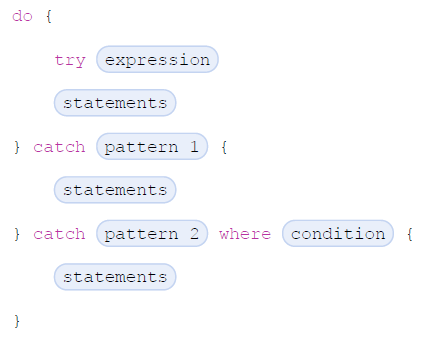
\includegraphics[height=8cm]{Images/doCatch.png}
    \caption{\textit{do-catch}-Anweisung in Swift \\ Quelle:\cite[S.314]{Apple.2017}}
    \label{fig:doCatchSwift}
\end{figure}

Wird ein Fehler im \textit{do}-Block geworfen, kann dieser Fehler in einem \textit{catch}-Block gefangen werden. 
Wird kein \textit{pattern} für einen \textit{catch}-Block definiert, fängt dieser \textit{catch}-Block jeden Fehler. 
\autoref{lst:doCatchSwift} zeigt die Anwendung einer \textit{do-catch}-Anweisung auf die Funktion aus \autoref{lst:ThrowingFunctionSWift}.

\begin{listing}[H]
\caption{\textit{do-catch}-Anweisung in Swift}
\label{lst:doCatchSwift}
\begin{SwiftCode}
do {
    try print(Divide(x: 6, y: 0))	
} catch MathErrors.DivisonByZero {	
    print("Error: y could not be Zero")
} catch {
    print("Error: Unknown Error")
}
\end{SwiftCode}
\end{listing}

Bei Aufruf der Funktion \textit{Divide} wird ein \textit{MathErrors.DivisonByZero}-Fehler geworfen, welcher im \textit{catch}-Block gefangen wird und die Meldung ,,Error: y could not be Zero'' ausgibt. 
Jeder andere Fehler wird im \textit{catch}-Block ohne Bedingung abgefangen und die Meldung ,,Error: Unknown Error'' ausgegeben.
Anschließend wird der Programmablauf fortgesetzt.

Laut \cite[S.181]{Hoffman.2017} gibt es bei der Arbeit mit Sprachen wie Java und C\# oftmals leere \textit{catch}-Blöcke. 
Swift beugt diesem Vorgehen mit dem \textit{try?}-Schlüsselwort vor. 
Das \autoref{lst:Try?Swift} zeigt die Anwendung des \textit{try?}-Schlüsselwortes.

\begin{listing}[H]
\caption{Anwendung des \textit{try?}-Schlüsselwortes in Swift}
\label{lst:Try?Swift}
\begin{SwiftCode}
//Klassische Anwendung ähnlich zu Java und C#
do {
    let result = try Divide(x: 6, y: 2) 
    print("Result: \(result)")
} catch {}

//Mit Verwendung des try?-Schlüsselwortes
if let result = try? Divide(x: 6, y: 2) {
    print("Result: \(result)")
}
\end{SwiftCode}
\end{listing}

Der Konstanten \textit{result} soll das Ergebnis des Funktionsaufrufs von \textit{Divide} zugewiesen und der Wert von \textit{result} ausgegeben werden. 
Zeile 2 - 5 zeigt die klassische Vorgehensweise ähnlich zu Java und C\# während in Zeile 8 - 10 das \textit{try?}-Schlüsselwort verwendet wird.
Nach Ansicht von \cite[S.181]{Hoffman.2017} macht die Verwendung von \textit{try?} den Quelltext übersichtlicher und einfacher lesbar.

In Java und C\# gibt es das Schlüsselwort \textit{finally} um beispielsweise nach einem \textit{try-catch}-Block abschließende Anweisungen auszuführen. 
Swift kennt hierzu das Schlüsselwort \textit{defer}.
\autoref{lst:deferSwift} zeigt die Anwendung des \textit{defer}-Schlüsselwortes.
Die Anweisung im \textit{defer}-Block (Zeile 5) wird am Ende der Ausführung des umschließenden Blocks (\textit{if-Fallunterscheidung in Zeile 2}) ausgeführt, sowohl im Normalzustand als auch bei einem Fehler oder vorzeitigen Verlassen der Funktion aufgrund des Schlüsselwortes \textit{return} oder \textit{break} \cite[S.317]{Apple.2017}.
Durch das \textit{defer}-Schlüsselwort ist es möglich, Aufgaben, die am Ende eines Blocks in jedem Fall auszuführen sind, an den Stellen im Quelltext zu platzieren, an der ihre Platzierung logisch ist.

\begin{listing}[H]
\caption{Anwendung von \textit{defer} in Swift \\ Quelle: \cite[S.318]{Apple.2017}}
\label{lst:deferSwift}
\begin{SwiftCode}
func processFile(filename: String) throws {
    if exists(filename) {
        let file = open(filename)
        defer {
            close(file)
        }
        while let line = try file.readline() {
            // Work with the file.
        }
        // close(file) is called here, at the end of the scope.
    }
}
\end{SwiftCode}
\end{listing}

Im \autoref{lst:deferSwift} ist dies beispielsweise die Methode \textit{close(file)} direkt nach dem Aufruf der Methode \textit{open(filename)}. 
Dieses Verhalten ist nicht nur im Fehlerfall interessant, sondern auch im Normalfall für die Strukturierung des Quelltextes. 

Wenn davon ausgegangen werden kann, dass eine \textit{throwing Function} oder auch Methode zur Laufzeit keinen Fehler wirft, kann das Schlüsselwort \textit{try!} verwendet werden.
In \autoref{lst:Try!Swift} wird die Verwendung des \textit{try!}-Schlüsselwortes veranschaulicht.

\begin{listing}[H]
\caption{Anwendung von \textit{try!} in Swift \\ Quelle: \cite[S.317]{Apple.2017}}
\label{lst:Try!Swift}
\begin{SwiftCode}
let photo = try! loadImage(atPath: "./Resources/John Appleseed.jpg")
\end{SwiftCode}
\end{listing}

Die Funktion von \autoref{lst:Try!Swift} wird von Apple folgendermaßen beschrieben:

\begin{quote}
\enquote{For example, the following code uses a  loadImage(atPath:) function, which loads the image
resource at a given path or throws an error if the image can’t be loaded. In this case, because the
image is shipped with the application, no error will be thrown at runtime, so it is appropriate to
disable error propagation.} \cite[S.317]{Apple.2017}
\end{quote}

Go bietet im Gegensatz zu Swift eine andere Art der Fehlerbehandlung.
In Go wird der \textit{error}-Typ benutzt, um einen Fehlerzustand zu kennzeichnen \cite[]{GoBlog.ErroHandling}.
\autoref{lst:ErrorBeispielGo} zeigt ein Beispiel für die Verwendung des \textit{error}-Typ in Go. 
%wie der \textit{error}-Type in Go verwendet wird.

\begin{listing}[H]
\caption{Beispiel für den \textit{error}-Typ in Go \\ Quelle:\cite[]{GoBlog.ErroHandling}}
\label{lst:ErrorBeispielGo}
\begin{GoCode}
func Open(name string) (file *File, err error)
\end{GoCode}
\end{listing}

Sollte beim Aufruf der Funktion \textit{Open} ein Fehler auftreten, gibt \textit{Open} einen Fehler in Form eines nicht leeren \textit{error}-Typs zurück.
\autoref{lst:ErrorBeispielGo2} zeigt die Anwendung des \textit{error}-Typs.

\begin{listing}[H]
\caption{Beispiel für die Anwendung des \textit{error}-Typs in Go \\ Quelle:\cite[]{GoBlog.ErroHandling}}
\label{lst:ErrorBeispielGo2}
\begin{GoCode}
f, err := os.Open("filename.ext")

if err != nil {
    log.Fatal(err)
}

// do something with the open *File f
\end{GoCode}
\end{listing}

In Zeile 3 wird überprüft, ob beim Aufruf der \textit{os.Open}-Funktion ein Fehler aufgetreten ist. 
Im Fehlerfall wird die Fehlermeldung ausgegeben und der Programmablauf abgebrochen.
Der Abbruch des Programms geschieht mit dem Aufruf der Funktion \textit{log.Fatal(err)}.
Die offizielle Dokumentation von Go äußert sich wie folgt zu dieser Funktion.

\begin{quote}
\enquote{Fatal is equivalent to Print() followed by a call to os.Exit(1).} \cite[]{GoDoc.Log}
\end{quote}

Auch Go besitzt die Fähigkeit eigene Fehler zu definieren.
Ein Beispiel hierfür ist in \autoref{lst:ErrorBeispielGo3} zu sehen.
Wird der Funktion \textit{Sqrt} ein negativer Wert übergeben, soll die Funktion den Wert 0 und den Fehler ,,math: square root of negative number'' zurück geben. 
Die Funktion \textit{New} aus dem Package \textit{errors} erzeugt eine neue Instanz vom Typ \textit{error}.

\begin{listing}[H]
\caption{Eigene Fehler in Go \\ Quelle:\cite[]{GoBlog.ErroHandling}}
\label{lst:ErrorBeispielGo3}
\begin{GoCode}
func Sqrt(f float64) (float64, error) {
    if f < 0 {
        return 0, errors.New("math: square root of negative number")
    }
    // implementation
}
\end{GoCode}
\end{listing}

\autoref{lst:ErrorBeispielGo4} zeigt, wie mit der Funktion \textit{errors.New} neue Fehler definiert werden können. 
Das Beispiel ist dem Quelltext von Go, im speziellen dem Package \textit{bufio} entnommen.

\begin{listing}[H]
\caption{Eigene Fehler in Go \\ Quelle:\cite[]{GolangBufio}}
\label{lst:ErrorBeispielGo4}
\begin{GoCode}
var (
    ErrInvalidUnreadByte = errors.New("bufio: invalid use of UnreadByte")
    ErrInvalidUnreadRune = errors.New("bufio: invalid use of UnreadRune")
    ErrBufferFull        = errors.New("bufio: buffer full")
    ErrNegativeCount     = errors.New("bufio: negative count")
)
\end{GoCode}
\end{listing}

Die in \autoref{lst:ErrorBeispielGo4} definierten Fehler können genutzt werden, um spezifische Fehler zu identifizieren. 
\autoref{lst:ErrorBeispielGo5} zeigt, wie die in \autoref{lst:ErrorBeispielGo4} definierten Fehler unterschieden werden können und unterschiedliche auf die Fehler reagiert werden kann.

\begin{listing}[H]
\caption{Unterscheidung von Fehlern in Go \\ Quelle:\cite[]{GoingGo.Error1}}
\label{lst:ErrorBeispielGo5}
\begin{GoCode}
data, err := b.Peek(1)
if err != nil {
    switch err {
        case bufio.ErrNegativeCount:
            // Do something specific.
            return
        case bufio.ErrBufferFull:
            // Do something specific.
            return
        default:
            // Do something generic.
            return
    }
}
\end{GoCode}
\end{listing}

Das Konzept zur Fehlerbehandlung von Swift ist dem anderer Programmiersprachen wie Java und C\# ähnlich und erweitert diese sogar mit weiteren Möglichkeiten.
Das Konzept von Go hingegen ist anders und erfordert für Entwickler, die beispielsweise mit Java vertraut sind, ein gewisses Umdenken bei der Behandlung von Fehlern. 
